  \documentclass[
    aps,
    reprint,
    superscriptaddress,
    %11pt
    ]{revtex4-2}
%\documentclass{article}
\usepackage[utf8]{inputenc}
\usepackage{kotex}
%\usepackage[HWP]{dhucs-interword}
%\usepackage[dvips]{color}
\usepackage{graphicx}
%\usepackage{bm}
\usepackage{amsmath}
%\usepackage{tikz}

\begin{document}
\title{그래픽 디자인과 물리학 : 블랙홀의 시각화}

\author{12181978 이휘재}
\affiliation{Physics Department, Inha University}

\date{\today}


\begin{abstract}
필자는 물리학과에 재학 중인 학부생으로 그래픽 디자인이 물리학에서 쓰인 사례 중, 개인적으로 가장
인상 깊었던 블랙홀에 대한 응용을 소개하고자 한다. 누구에게나 블랙홀을 간략하게 그려보라면
그리지 못할 사람이 없겠지만, 블랙홀의 실제 모습을 담은 사진이 2019년에서야 처음으로 찍혔다는 
사실은 잘 알려져 있지 않을 것이다. 그럼에도 대중들이 블랙홀의 모습을 친숙하게 생각하는 
이유가 컴퓨터를 이용한 그래픽 디자인에 있다고 생각하여, 필자는 제목과 같이 주제를 정하게 되었다.  
\end{abstract}

\maketitle

\section[Introduction]{소개}
2019년 EHT(Event Horizon Telescope)에서 출판한 논문 'First M87 Event Horizon Telescope Results. I.
The Shadow of the Supermassive Black Hole'은 인류 역사상 처음으로 블랙홀을 직접 관측한 방법과
그 사진이 담겨있다. 다시 말하면 이 논문이 출판되기 전까지 존재하던 모든 블랙홀 사진, 그림들은
모두 사람이 직접 그렸거나 컴퓨터 그래픽을 통해 만들어내었다고 볼 수 있다. 블랙홀이 존재한다는 사실과
블랙홀의 정확한 위치까지 알고 있었지만, 블랙홀을 직접 관측할 기술이 없었던 것이다. 극단적으로 말하자면, 
우리가 흔히 블랙홀이라고 생각해왔던 모습들은 전부 가짜였다. 하지만 우리가 과학자들에게 속았다고
속단할 수는 없다. 
아인슈타인이 일반 상대성 이론으로 그 시작을 마련한 블랙홀 연구에 슈바르츠실트, 찬드라세카르, 
펜로즈와 호킹 등이 커다란 기여를 보태면서, 과학자들은 블랙홀이 만들어내는 블랙홀 주변 시공간의 
변화를 계산해낼 수 있었고, 이 노력들이 현대시대에 들어 급격히 발전해온 컴퓨터 그래픽 기술을
만나 과학자들이 상상하던 블랙홀을 볼 수 있게 되었다. 과학자들이 보여주던 블랙홀 사진이 완전한 허구는 
아니였던 것이다. 그 사진들은 검증된 수식과 컴퓨터의 연산으로 만들어진 일종의 작품이었다.

\section{물리학에서 바라본 블랙홀}
질량이 존재하면 중력이 존재하고 질량이 크면 중력도 크다. 그 중력은 질량의 중심 방향으로 향하기 때문에 
지구에서 사람이 벗어날 때 로켓의 힘을 빌리는 것처럼 빠른 속도로 중력의 영향을 벗어나야 한다. 
블랙홀은 질량이 매우 커서 이 속도가 빛의 속도보다 빨라야 하는 천체이다. 하지만 이 우주에서 빛보다 빠른 
것은 없으므로 블랙홀을 빠져나갈 수 있는 무언가는 존재하지 않는다. 물론 블랙홀의 종류에 따라 입자가 빠져나올
수도 있다. 하지만 블랙홀의 중력장에 어느정도 강하게 잡혀버리면 탈출하는 방법은 블랙홀에 빨려들어 갔다가
입자단위로 분해되어 방출되기를 기다리는 것 뿐이다.
또한 중력은 거리가 가까울 수록 강해진다. 그래서 블랙홀에 너무 가까이만 가지 않으면 블랙홀에 빨려 들어가지
않을 수 있다. 어느 정도 가까워지면 탈출에 필요한 속도가 광속보다 빨라지는데 이 영역을 사건의 지평선(The
event horizon)이라고 부른다. \\
그런데 중력은 왜 발생하는 것일까? 아인슈타인은 중력을 시공간의 휘어짐으로 설명했다. 
아인슈타인의 일반 상대성 이론에 따르면 시공간에 질량이 존재하면 그 질량이 시공간을 휘어지게 만들어 
중력이 작용하는 것처럼 보이게 한다. 시공간이 휘어지면 그 주변에 위치한 물체들이 휘어진 시공간을 
따라 움직이는데 이것이 중력이 작용하여 끌어당겨지는 것처럼 보이게 된다. 빛이 대표적인 예이다. 
빛은 직진하는 성질을 가지고 있는데 휘어진 시공간에서는 그 경로가 휘어진다. 빛 스스로는 직진하고 
있는데 말이다. 이는 마치 우리가 A4 용지에 자를 대고 직선을 그려도 A4 용지를 구부려 보면 직선이 
곡선으로 보이는 것과 같은 이치이다.
시공간이라 표현한 이유는 공간 뿐만 아니라 시간의 흐름 또한 휘어지게 하기 때문이다. 
시공간이 많이 휘어져 있을 수록 물체는 더 강하게 끌어당겨질 뿐만 아니라, 시간 또한 천천히
가게 된다. 블랙홀은 이 시공간을 굉장히 많이 휘어지게 만드는 천체인 것이다.  \\
블랙홀을 직접 관측하기 어려운 이유가 여기에 있다. 우선 블랙홀은 너무 멀리 있어 관측장비의 성능이 
굉장히 좋아야 한다. 지구와 가장 가까이 위치한 궁수자리 20A 블랙홀은 태양계로부터 
27000광년 만큼 떨어져 있다. 27000광년은 27000년 동안 광속으로 움직였을 때 도달하는 거리이다.
좋은 관측장비로 블랙홀의 위치를 파악하더라도 빛을 빨아들이기 때문에 볼 수 조차 없다.
과학자들이 발견했다고 하는 블랙홀도 직접 보고 판단한 것이 아니라 블랙홀이라 의심되는 천체로부터 
빠져나온 입자, 에너지를 보고 블랙홀이겠구나 하고 의심하는 것이다. 후속적인 연구가 성공적으로 
이어져야 블랙홀이라는 확신을 가질 수 있다.

\section{컴퓨터 그래픽으로 만들어낸 블랙홀}
영화 인터스텔라를 본 사람이라면 이미 컴퓨터 그래픽으로 만들어진 블랙홀 '가르강튀아'를 통해
블랙홀이 눈 앞에 놓여진 모습을 생생히 기억할 것이다. 영화 인터스텔라는 블랙홀을 가까이 있는 누군가가
볼 수 있는 것처럼 묘사하려고 시도한 최초의 할리우드 영화이다. 이를 위해 Double Negative
Visual Effects 팀과 물리학자 킵 손(Kip Thorne)
%\footnote{킵 손은 중력파 관측에 대한 공로로 2017년 노벨 물리학상을 수상하였다. }
이 공동으로 작업하여 
DNGR(Double Negative Gravitational Renderer)이라 부르는 코드를 개발하였다. 
DNGR은 블랙홀 주위 휘어진 시공간을 지나는 빛 다발의 궤적을 IMAX 규격에 맞게 시각화하는 코드로
DNGR의 길이는 4만줄에
달하며 C++언어로 작성되었다. DNGR을 이용해 IMAX 규격으로 제작된 인터스텔라의 블랙홀 이미지 단 1장을 
만드는데 10개의 CPU 코어를 사용하여 대략 수시간이 걸린다. 이렇게 만들어낸 이미지가 수없이 많이 모여
영화에 등장한 것이다. 블랙홀의 이미지를 만들어내는데 이렇게나 긴 코드와 많은 시간이 필요한 이유는
휘어진 시공간을 표현하는 수식에 있다.  
\begin{figure}[htp]
  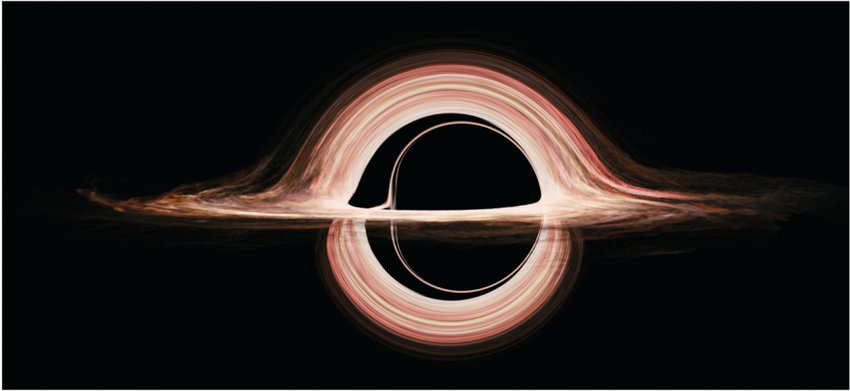
\includegraphics[scale=1]{interstellar.png}
  \caption{DNGR을 이용한 블랙홀과 현실적인 강착원반의 시각화\cite{Janes}}
  \label{fig:5}
\end{figure}

휘어진 시공간을 표현하는데 기본이 되는 아인슈타인 장 방정식은 다음과 같다.
\begin{align}
  G_{\mu\nu} + \Lambda g_{\mu\nu} = \kappa T_{\mu\nu},\,\,\,
  G_{\mu\nu} = R_{\mu\nu} -\frac{1}{2}Rg_{\mu\nu}
\end{align}
이 수식에 등장하는 $G_{\mu\nu},g_{\mu\nu},T_{\mu\nu},R_{\mu\nu}$는 수학과 물리학에서 
텐서(tensor)라 부르는 양으로 아랫 첨자들 $\mu, \nu$가 정해지면 하나의 변수가 된다. 쉽게 말하면
이 텐서들은 $4\times 4$ 행렬과 같다. 즉, 하나의 텐서에 16개의 미지수가 존재하는 것이다.
그런 텐서가 4개 등장하고 하나는 다른 두 텐서로 표현되므로 이 방정식은 세개의 텐서로 표현이 가능하다.
다시 말하자면, 이 수식 하나에 미지수 $16\times 3 = 48$개가 등장한다. 따라서 이 수식에 특별한 
조건들을 부여하여 미지수의 개수을 줄이지 않는 이상 손으로 방정식을 푸는 것은 불가능하다. 
DNGR은 블랙홀의 위치, 질량과 회전속력, 카메라의 위치와 속도, 시선 각도에 추가적인 요소들을
고려하여 블랙홀 이미지의 한 픽셀에 보여질 결과를 연산하는 것이다. 이와 같은 복잡한 과정을 거쳐
만들어낸 블랙홀의 이미지는 아인슈타인의 일반 상대성 이론이 수식으로 서술한 블랙홀을 눈으로
볼 수 있게 해준다. \\
인터스텔라의 가르강튀아와 같이 정교한 이론과 컴퓨터 기술로 시각화된 블랙홀을 NASA에서도 접할 수 
있다. NASA's Goddard Space Filght Center의 Jeremy Schnittman이 제작한 이 시각화는 
블랙홀을 여러 시점으로 바라본 영상들을 제공해주고 GIF파일로 다운로드를 받을 수도 있다.
\begin{figure}[htp]
  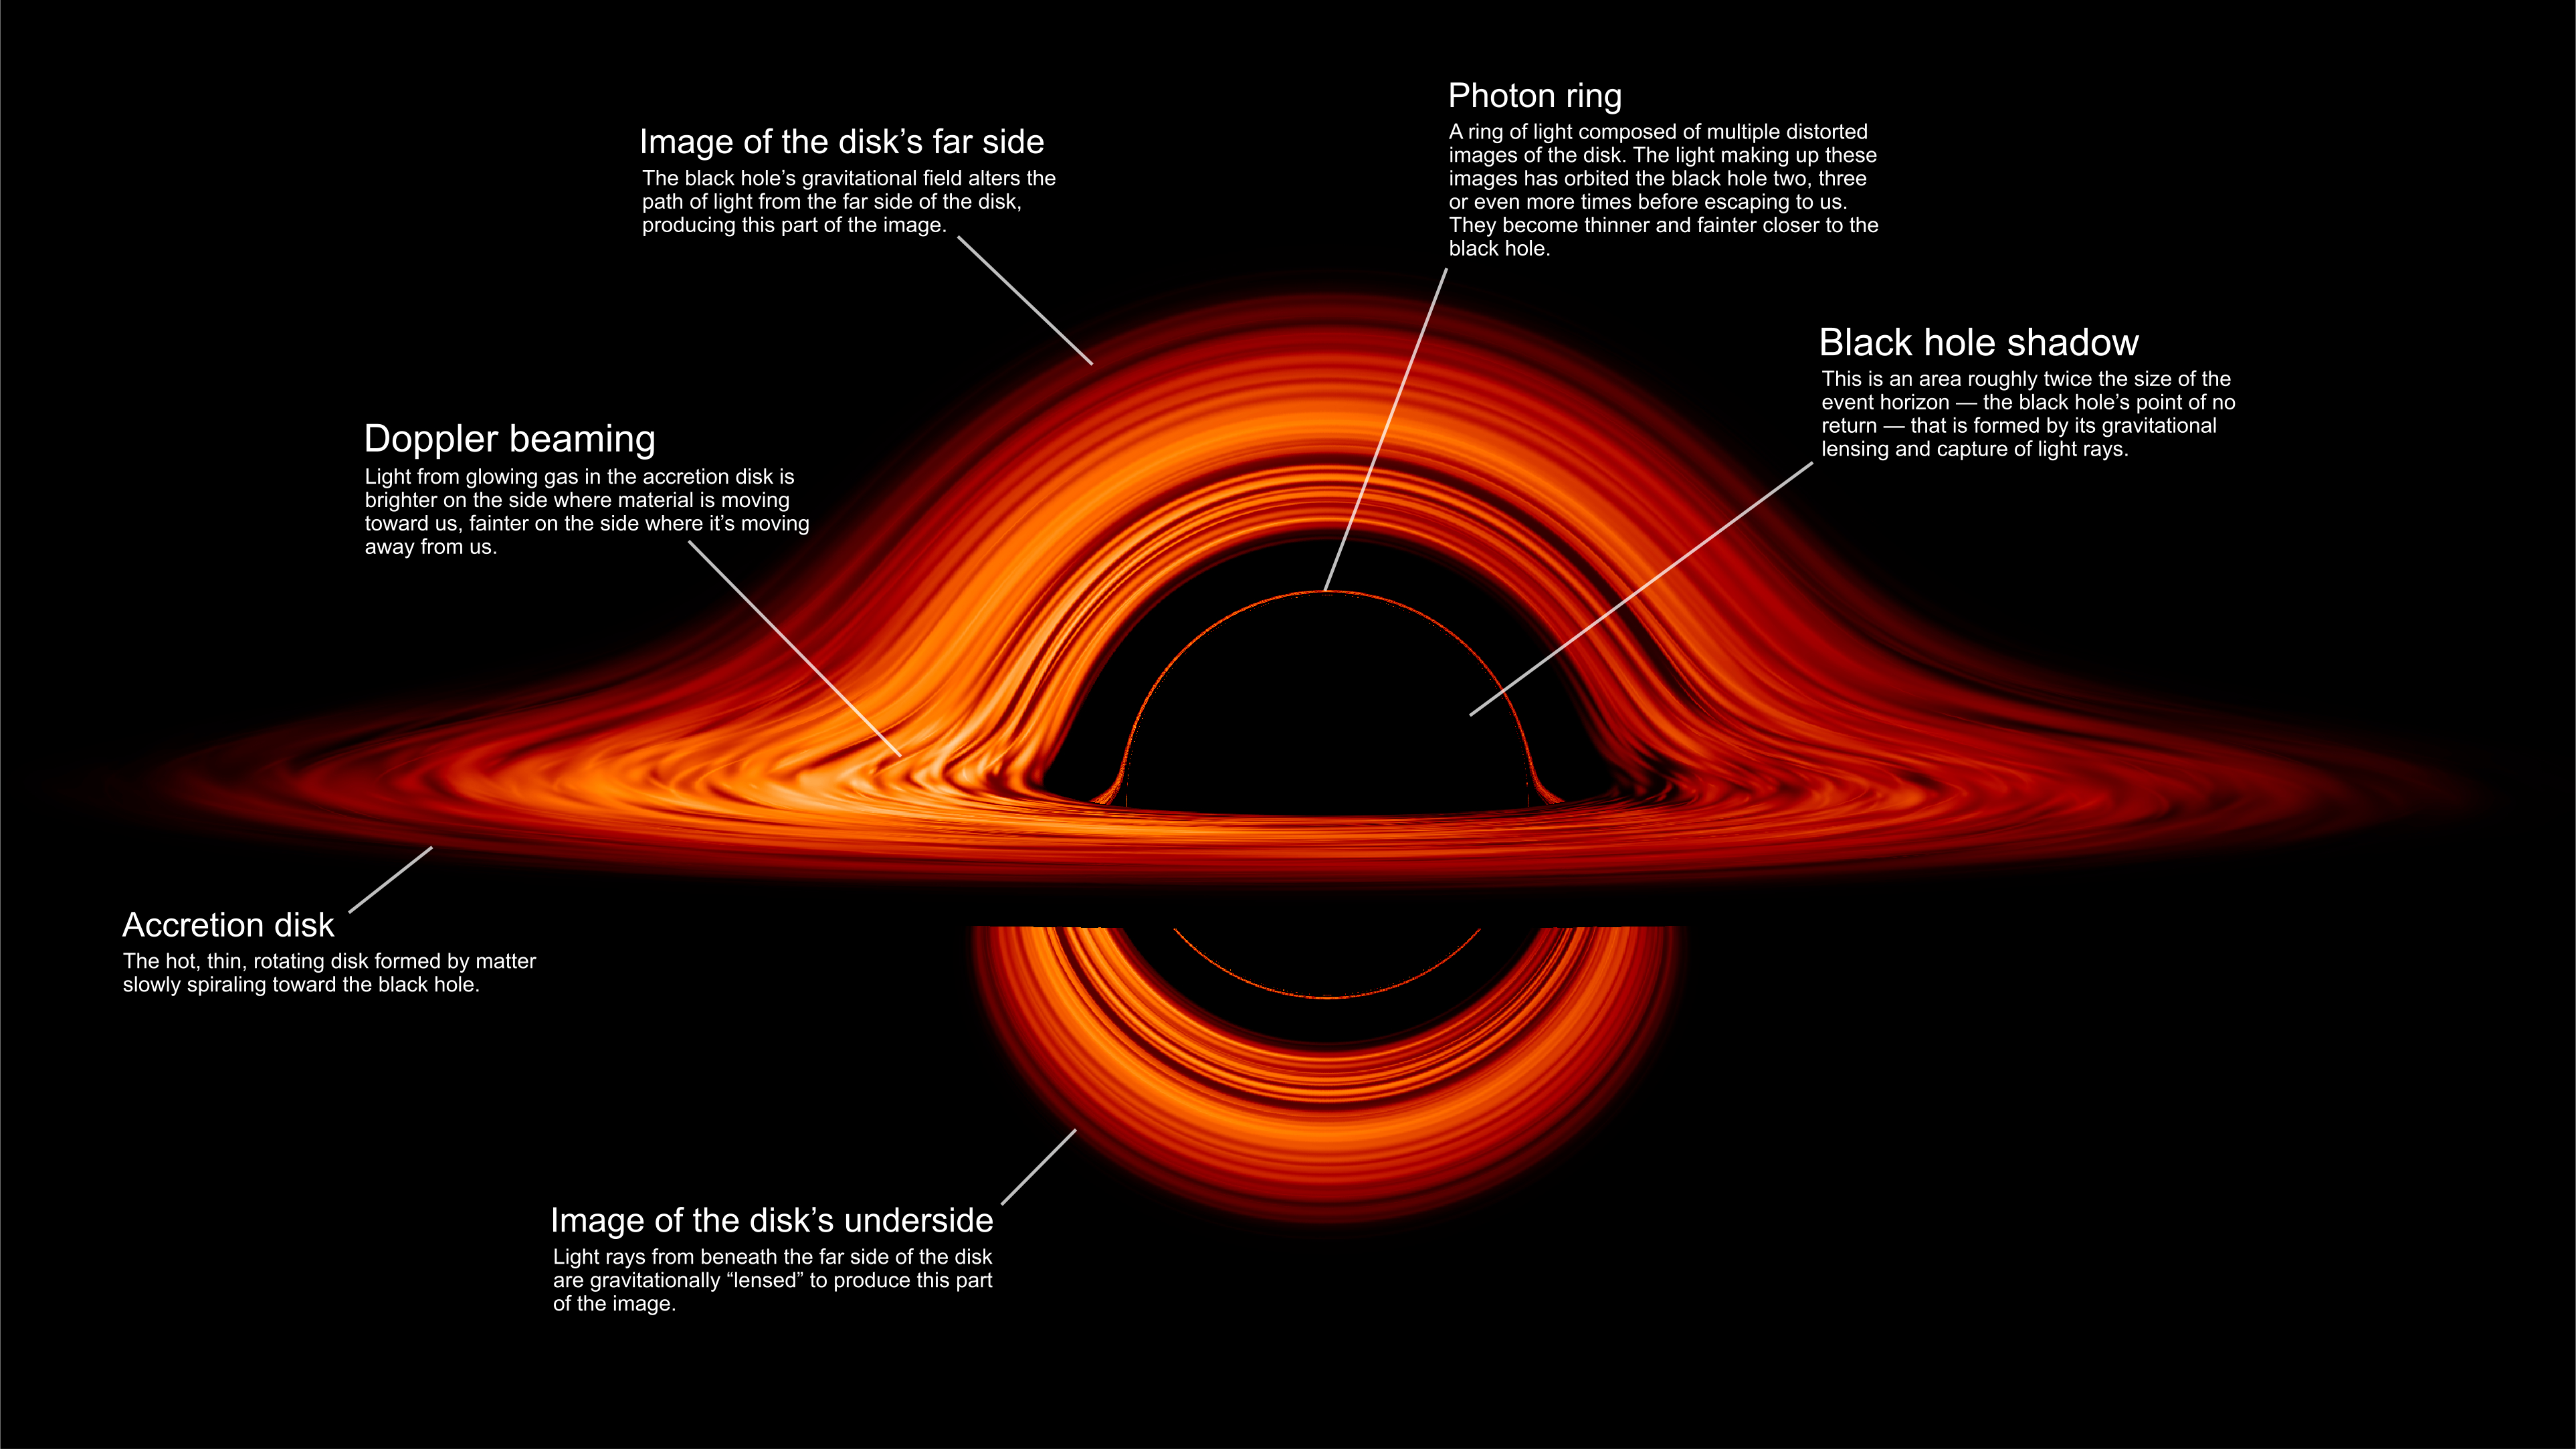
\includegraphics[scale=0.08]{nasa.jpg}
  \caption{NASA에서 제공하는 시각화된 블랙홀과 그에 대한 설명}
  \label{fig:6}
\end{figure}
이 영상들을 통해 블랙홀 주변에서 시공간이 어떻게 휘어지는지, 블랙홀을 가까이서 관측했을 때 
휘어진 시공간으로 인해 우리의 눈에 들어올 광경을 영화보다 더 자세히 볼 수 있다.
\nocite{*}
\bibliography{ref}



%\begin{thebibliography}{9}
%\end{thebibliography}

%\vfill
\end{document}